\lstset{language=bash}
\newpage
\chapter{Background}
\label{chap:background}
% ==============================================================================
\section{What is a Version Control System}
\noindent
A \acrfull{vcs} saves modifications made by individual software developers, allowing them to track their work over time and making the process more accessible. Furthermore, it facilitates sharing data between nodes, where each node can be kept up to date with the latest versions, minimising the need to handle merge conflicts.
\smallskip

\acrlongpl{vcs} provide several advantages, such as aiding in collaboration among programmers and improving efficiency when working on large groups of mixed products. In addition, \acrshortpl{vcs} offer an audit trail and easy branching functionality, simplifying team-based development. It also enables an understanding of who has worked on specific pieces or sections during a given period.
\smallskip

By ensuring all changes are appropriately tracked, \acrshortpl{vcs} promote transparency within teams while maintaining optimal performance levels through streamlined management processes. This helps avoid errors arising from inconsistencies between versions, such as mismatched documents or programming problems resulting from conflicting edit operations.

\paragraph{Significance of Version Control Systems}
\hfill\medskip\\
For most software projects, the source code is a valuable asset that must be protected. Additionally, for many software teams, the source code represents a repository of invaluable knowledge and understanding about the problem that developers have amassed and refined through meticulous effort.
\smallskip

Version control safeguards this precious resource by preventing catastrophes, casual degradation, human error, or unintended consequences from affecting its quality. Software developers working in teams continually write new source code and modify existing code, which is organised into file folders called "file trees". Developers may work on different tasks simultaneously, such as implementing new features or fixing unrelated bugs, by altering parts of the file tree.
\smallskip

Version control assists teams in addressing these challenges by tracking each change made by contributors, helping to prevent concurrent work from conflicting with one another. Consequently, any incompatibility can be detected and resolved without impeding team members' progress further down the line, ensuring that changes do not introduce bugs.

\section{Evolution of Version Control Systems}
\noindent
\begin{figure}[htbp]
    \centering
    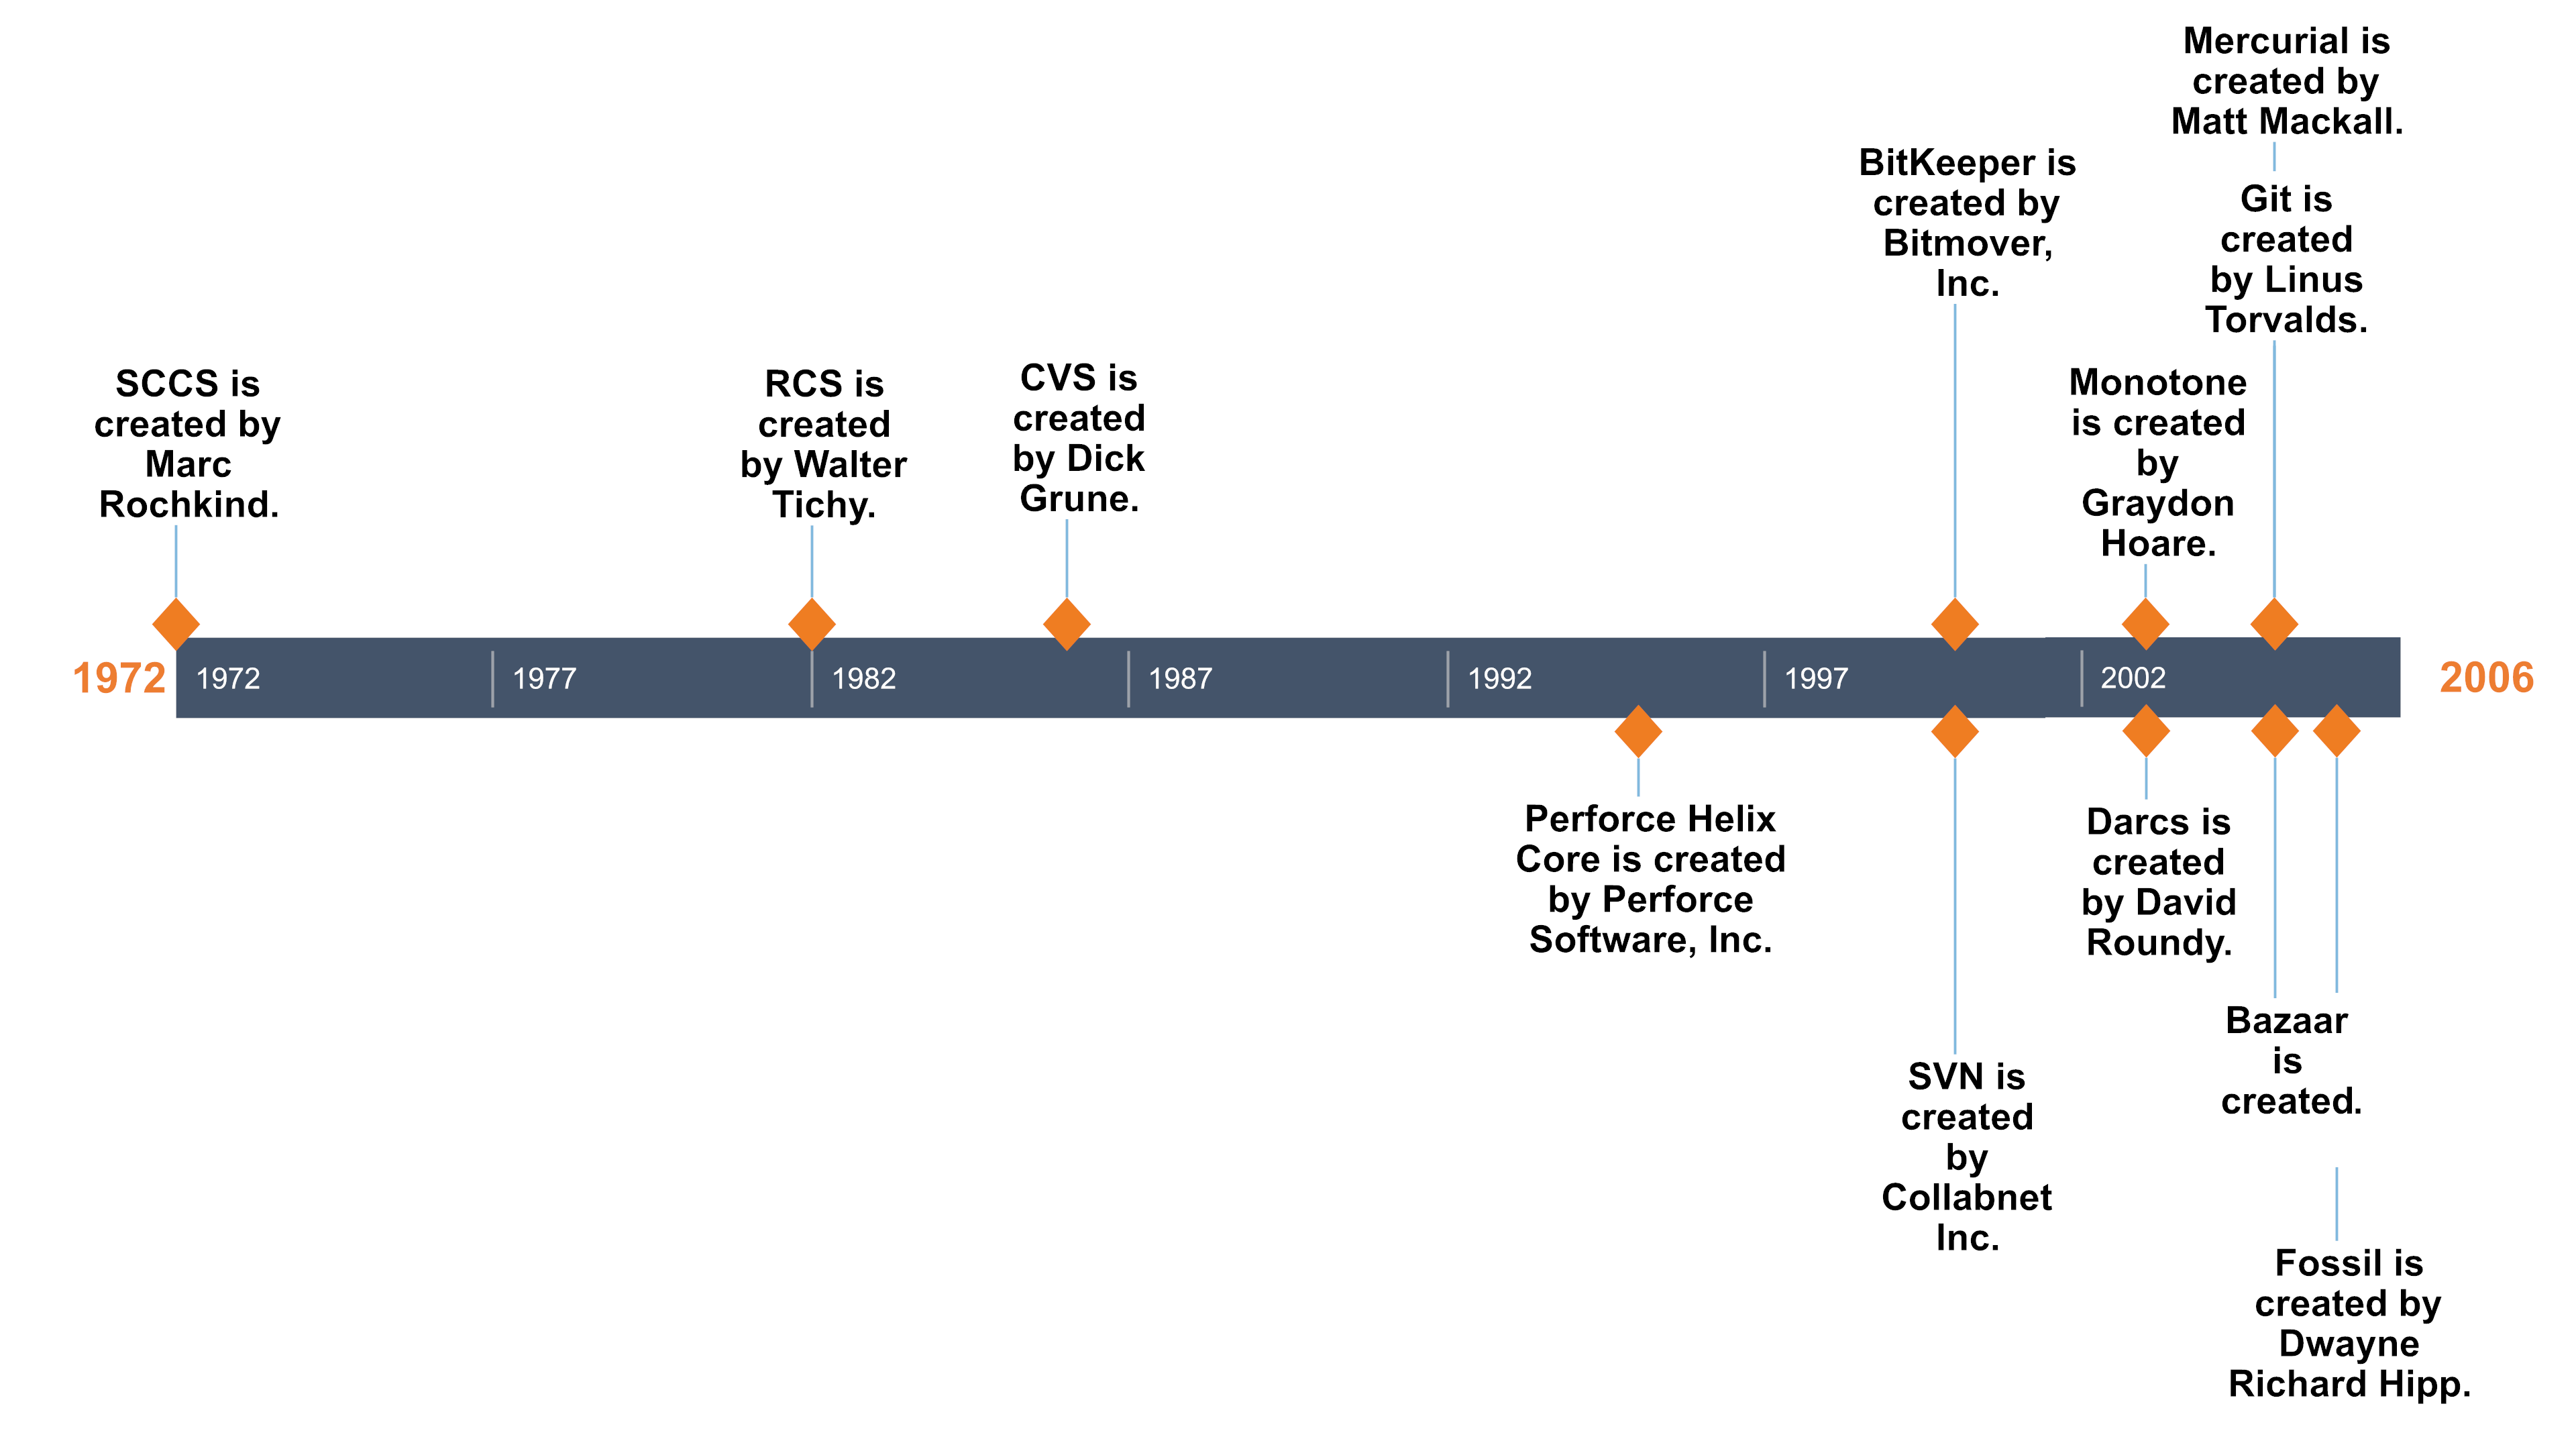
\includegraphics[width=0.95\textwidth]{vcs-timeline.png}
    \caption{Timeline of the Creation of Version Control Systems \cite{stopak_2019}}
    \label{fig:vcs-timeline}
\end{figure}
\subsection{Local Version Control Systems (LVCS)}
Local Version Control Systems are systems designed to operate on a single machine, early VCSs were intended to track changes for individual files, and checked-out files could only be edited locally by one user at a time \cite{stopak_2019}. In addition, they were built on the assumption that all users would log into the same shared Unix host with their own accounts, which was not always possible.
\smallskip

The main benefit of LVCS is that it provides a basic level of version control functionality without requiring any network connectivity. However, this can also be seen as a drawback when you consider that with LVCS, there is no central repository to store the code, which means that each developer has their own copy. This can lead to issues with merging changes and tracking changes across multiple copies.

\begin{figure}[htbp]
    \centering
    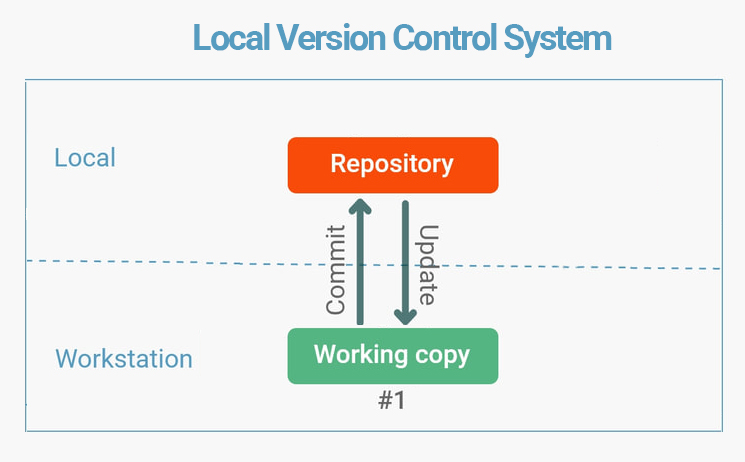
\includegraphics[width=0.8\textwidth]{local-vcs-structure}
    \caption{Local Version Control System (LVCS)}
    \label{fig:lvcs-structure}
\end{figure}

\subsubsection{Source Code Control System (SCCS)}
\label{sec:sccs}
\acrlong{sccs} was released in 1972 and is one of the first successful \acrshort{vcs} tools \cite{stopak_2019}. It was written by Marc Rochkind at Bell Labs, who wanted to solve the problem of tracking file revisions. The tool made tracking down bugs introduced into a program significantly more manageable. \acrshort{sccs} is worth understanding at a basic level because it helped set up modern \acrshort{vcs} tools that developers use today.
\paragraph{Architecture}
\hfill\medskip\\
% Much like modern VCS tools, SCCS has a set of commands that allow developers to work with versioning of files. The basic command functionality are:
Much like modern \acrshort{vcs} tools, \acrshort{sccs} has a set of commands that allow developers to work with the versioning of files. The basic command functionality is:
\begin{itemize}
    \item Check-in files to track their history.
    \item Check-out specific file versions for review.
    \item Check-out specific file versions for editing.
    \item Check-in new file versions with comments explaining the changes.
    \item Revert changes made to a checked-out file.
    \item Basic branching and merging of changes.
    \item Print a log of a file's version history.
\end{itemize}
% A special type of file called a \lstinline{s-file} or a \lstinline{history file} is created when a file is tracked by SCCS. This file is named with the original filename prefixed with a \lstinline{s.}, and is stored in a subdirectory called \lstinline{SCCS}.
A particular type of file called an \lstinline{s-file} or a \lstinline{history file} is created when a file is tracked by SCCS. This file is named with the original filename prefixed with an \lstinline{s.} and is stored in a subdirectory called \lstinline{SCCS}.
\smallskip

So a file called \lstinline{test.txt} would get a history file created in the \lstinline{./SCCS/} directory with the name of \lstinline{s.test.txt}. When created, the \lstinline{s-file} contains the original file contents, a header that contains the file's version number, and some other metadata. There are also checksums stored in the \lstinline{s-file} that are used to verify the integrity of the file (i.e. to ensure that the file has not been tampered with). The \lstinline{s-file} content is not encoded or compressed in any way, which is a clear difference from modern VCS tools.
\smallskip

Since the original file's content is now stored in the history file, it can be retrieved into the working directory for review, compilation, or editing. Further changes made to this new copy, such as line additions, modifications and removals, can be checked back into a revised version of the history file, which increments its revision number \cite{stopak_2019}.
\smallskip

Subsequent SCCS check-ins only store only deltas or changes to a file instead of storing entire contents each time; when a check-in is made, subsequent revisions are added onto existing delta tables inside an amended history file (history files do not use compression). This decreases the size of these large histories since they are not using compression on their files, so they take up more space than just having one complete copy that you are tracking with no differences like Word docs etc.

% TODO: 2023-04-18
% \smallskip

% As previously mentioned, SCCS uses the Delta method known as Interleaved Deltas, which allows constant-time checkout regardless of how old your checked-out revision is - i.e., older revisions do not take longer than newer ones.
% \smallskip

% It is important to note that all files are tracked and checked in separately; there is no way to check in changes on multiple files as a part of one atomic unit - like a commit in \nameref{sec:git}. Each tracked file has its corresponding history file, which stores revisions. Generally, this means that the version numbers of different files cannot match each other. However, matching revision numbers can be achieved by editing every file at once (even if not all of the changed areas have fundamental changes) and checking them all together. This will increment revision numbers for any modified content, so they will be consistent with their revisions—but it's not comparable to including lots of different pieces within a single commit like you would in \nameref{sec:git}. In SCCS, these make individual check-ins across separate history folders rather than one extensive report containing everything at once.
% \smallskip

% When a file is checked out for editing in SCCS, it is locked so that anyone else cannot edit it. This prevents changes from being overwritten by other users and limits development since only one user can edit the file simultaneously.
% \smallskip

% The software supports branches that store sequences of changes to specific files - these can then be merged back into the original versions or with copies of other branched versions of the same parent branch.

% TODO: Consider adding command examples
% \paragraph{Basic Commands}

% \begin{itemize}
%     \item \lstinline{sccs create <filename.ext>} - Check in a new file to SCCS and create a new history file for it (in the \lstinline{./SCCS/} directory by default).
%     \item \lstinline{sccs get <filename.ext>} - Check out a file from from its corresponding history file and place it in the working directory in readonly mode.
%     \item \lstinline{sccs edit <filename.ext>} - Check out a file from the corresponding history file for editing. Locks the history file so no other users can modify it.
%     \item \lstinline{sccs delta <filename.ext>} - Check in the modifications to the specified file. Will prompt for a comment, store the changes in the history file, and remove the lock.
%     \item \lstinline{sccs prt <filename.ext>} - Display the revision log for a tracked file.
%     \item \lstinline{sccs diffs <filename.ext>} - Display the differences between the current working copy of a file and the state of the file when it was checked out.
% \end{itemize}

\subsubsection{Revision Control System (RCS)}
\label{sec:rcs}
The \acrlong{rcs} was released in 1982 as an alternative to the closed-source \acrlong{sccs}. Developed by Walter Tichy and written in C, \acrshort{rcs} was released under the GNU General Public License, making it suitable for use in open-source projects.

\begin{quote}
    "\acrshort{rcs} manages revisions of text documents, in particular source programs, documentation, and test data. It automates the storing, retrieval, logging and identification of revisions." -- Walter Tichy \cite{tichy_1985}
\end{quote}

\paragraph{Architecture}
\hfill\medskip\\
RCS shares many traits with its predecessor\cite{stopak_2019}, including:
\begin{itemize}
    \item Handling revisions on a file-by-file basis.
    \item Changes across multiple files can't be grouped together into an atomic commit.
    \item Tracked files are intended to be modified by one user at a time.
    \item No network functionality.
    \item Revisions for each tracked file are stored in a corresponding history file.
    \item Basic branching and merging of revisions within individual files.
\end{itemize}

Upon checking a file into RCS for the first time, a corresponding history file is created in the local \lstinline{./RCS/} directory. The history file is postfixed with a \lstinline{,v}, so a file named \lstinline{test.txt} would be tracked by a file called \lstinline{test.txt,v}\cite{stopak_2019}.
\smallskip

\acrshort{rcs} employs a reverse-delta scheme for storing file changes. When a file is checked in, the history file contains a complete snapshot of its contents. Subsequent modifications and check-ins result in RCS calculating a single delta—the difference between the new version of that specific revision and the previously recorded version - and saving it along with an older snapshot if necessary.

% TODO: 2023-04-18
% \smallskip

% The reverse-delta scheme functions by checking out an earlier revision from the newest version and applying consecutive deltas until reaching the desired revision. Starting from the newest version allows quick checkout times, as the current revisions' snapshots are readily accessible.
% \smallskip

% However, when attempting to access older versions beyond just one recent update (e.g., 1 or 2 old versions), the process becomes considerably more complex. This is because these older versions' snapshots must be calculated against each other before they can be applied to the newest version.
% \smallskip

% Unlike RCS, SCCS maintains a consistent checkout time for any revision. Additionally, RCS history files do not store checksums, meaning file integrity cannot be guaranteed.

% TODO: Consider adding command examples
% \paragraph{Basic Commands}

% \begin{itemize}
%     \item \lstinline{ci <filename.ext>} - Check in a new file to RCS and create a new history file for it (in the \lstinline{./RCS/} directory by default).
%     \item \lstinline{co <filename.ext>} - Check out a file from from its corresponding history file and place it in the working directory in readonly mode.
%     \item \lstinline{co -l <filename.ext>} - Check out a file from the corresponding history file for editing. Locks the history file so no other users can modify it.
%     \item \lstinline{ci <filename.ext>} - Check in file changes and create a new revision for it in its corresponding history file.
%     \item \lstinline{merge <file-to-merge-into.ext> <parent.ext> <file-to-merge-from.ext>} - Merge changes from two modified children of the same parent file.
%     \item \lstinline{rcsdiff <filename.ext>} - Display the differences between the current working copy of a file and the state of the file when it was checked out.
%     \item \lstinline{rcsclean} - Removes working files that don't have locks on them.
% \end{itemize}

\subsection{Centralized Version Control Systems (CVCS)}
\label{sec:cvcs}
A Centralised Version Control System is a system that enables developers to work together on the same project by storing the primary copy of files in a central repository. This system keeps track of all files and saves information in the local repository. CVCS is called centralised because there is only one central server or repository.
\smallskip

The server maintains a complete record of issues, while clients only maintain a local copy of the shared documents. All developers make their modifications to the repository through checkout. However, only the last version of the files is retrieved from the server, meaning any modifications made will automatically be shared with other developers.
\smallskip

Users can modify in parallel with their local copy of shared documents and sync with the central server to release their contributions and make them visible to other collaborators. However, because centralised version control systems rely on one repository that includes the correct project version, they must restrict write access so that only trusted contributors can commit modifications.
\smallskip

CVCS has some challenges, such as if the central server is inaccessible, users cannot merge their work or save the released modifications. Also, if the central repository is corrupted, everything will be lost. Contributors must be the ones who have writing permissions to perform basic tasks, such as reverting modifications to a previous state, creating or merging branches, or releasing modifications with complete revision history. This limitation affects participation and authorship for new contributors.
\smallskip

So, the main drawbacks of using CVCS are that it requires a network connection to work on the source code, developers must order to contribute to a project, and a single point of failure is an issue when using one server.

% \begin{figure}[htbp]
\begin{figure}[H]
    \centering
    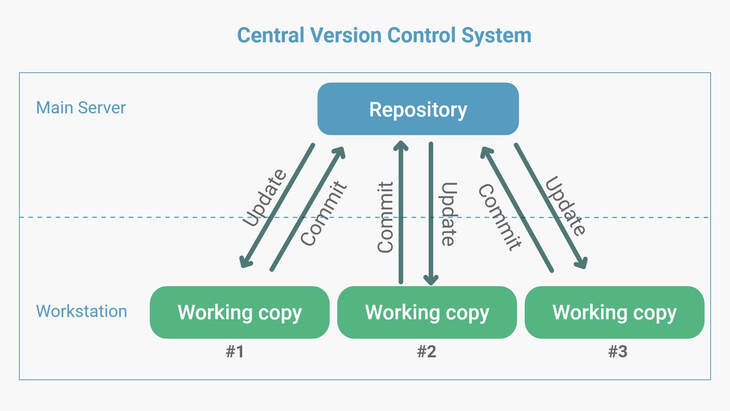
\includegraphics[width=0.85\textwidth]{centralized-vcs-structure}
    \caption{Centralized Version Control System (CVCS)}
    \label{fig:cvcs-structure}
\end{figure}

\subsubsection{Concurrent Versions System (CVS)}
\label{sec:cvs}
Dick Grune developed the Concurrent Versions System in 1986 to introduce a networking element to version control. Written in \lstinline{C}, CVS became the first widely used VCS tool that enabled multiple users to work on the same project simultaneously from different locations. This innovation began the second generation of VCS tools and facilitated collaboration among geographically dispersed development teams.
\paragraph{Architecture}
\hfill\medskip\\
CVS functions as a frontend for RCS, providing a set of commands to interact with files in a project while utilising the RCS history file format and commands behind the scenes. CVS allowed multiple developers to check out and work on duplicate files for the first time in history by employing a centralised repository model.
\smallskip

When a project is imported into CVS, each file is converted into a \lstinline{,v} history file and stored in a central directory referred to as a \lstinline{module}\cite{stopak_2019}. Generally, the repository resides on a remote server accessible via a local network or the Internet.
\smallskip

A developer checks out a copy of the module, which is copied to a working directory on their local machine. No files are locked during this process, allowing an unlimited number of developers to check out the module simultaneously. In addition, developers can modify their checked-out files and commit changes as needed.
\smallskip

When a developer commits a change, other developers must update their working copies through a (usually) automated merge process before committing their changes. Occasionally, merge conflicts require manual resolution before a commit can be made. Therefore, CVS also offers the capability to create and merge branches.

% TODO: Consider adding command examples
% \paragraph{Basic Commands}

% \begin{itemize}
%     \item \lstinline{export CVSROOT=<path/to/repository>} - Sets the CVS repository root directory so it doesn't need to be specified in each command.
%     \item \lstinline{cvs import -m 'Import module' <module-name> <vendor-tag> <release-tag>} - Import a directory of files into a CVS module. Before running this browse into the root directory of the project you want to import.
%     \item \lstinline{cvs checkout <module-name>} - Copy a module to the working directory.
%     \item \lstinline{cvs commit <filename.ext>} - Commit a changed file back to the module in the central repository.
%     \item \lstinline{cvs add <filename.txt>} - Add a new file to track revisions for.
%     \item \lstinline{cvs update} - Update the working copy by merging in committed changes that exist in the central repository but not the working copy.
%     \item \lstinline{cvs status} - Show general information about the checked out working copy of a module.
%     \item \lstinline{cvs tag <tag-name> <files>} - Add an identifying tag to a single file or set of files.
%     \item \lstinline{cvs tag -b <new-branch-name>} - Create a new branch in the repository (must be checked out before working on it locally).
%     \item \lstinline{cvs checkout -r <branch-name>} - Checkout an existing branch to the working directory.
%     \item \lstinline{cvs update -j <branch-to-merge>} - Merge an existing branch into the local working copy.
% \end{itemize}

% ==============================================================================
\subsubsection{Perforce Helix Core}
\label{sec:perforce}
Perforce Helix Core is a proprietary VCS developed, owned, and maintained by Perforce Software Inc., Written in \lstinline{C} and \lstinline{C++}; it was initially released in 1995. Although primarily designed for a centralised model, it also offers a distributed model option. Helix Core is commonly used by large companies managing substantial content with large binary files, such as in the video game development industry. Although typically cost-prohibitive for smaller projects, Perforce provides a free version for teams of up to five developers.
\paragraph{Architecture}
\hfill\medskip\\
Perforce Helix Core utilises a server/client model. The server, a process called \lstinline{p4d}, listens for incoming client connections on a designated port, typically port \lstinline{1666}. The client, a process called \lstinline{p4}, is available in both command-line and GUI variants. Users run the \lstinline{p4} client to connect to the server and issue commands. Support for various programming language APIs, including Python and Java, enables automated issuance and processing of Helix Core commands via scripts. Integrations are also available for IDEs like Eclipse and Visual Studio, allowing users to work with version control within those tools.
\smallskip

The Helix Core Server manages repositories called depots, which store files in directory trees similar to \nameref{sec:svn}. Clients can check out sets of files and directories from the depots into local copies called \lstinline{workspaces}. The atomic unit used to group and track changes in Helix Core depots is called the \lstinline{changelist}, which is analogous to Git commits. In addition, Helix Core implements two similar forms of branching: \lstinline{branches} and \lstinline{streams}. While branches represent separate lines of development history, a stream is a branch with added functionality that Helix Core uses to provide recommendations on best merging practices throughout the development process.
\smallskip

When a file is added for tracking, Helix Core classifies it using a \lstinline{file type} label. The two most commonly used file types are text and binary. For binary files, the entire file content is stored each time the file is saved. This is a common VCS tactic for handling binary files, which are not amenable to the normal merge process, as manual conflict resolution is typically impossible.
\smallskip

Only the deltas (changes between revisions) are stored for text files. Text file history and deltas are stored using the \nameref{sec:rcs} format, which tracks each file in a corresponding \lstinline{,v} file in the server depot. This is similar to \nameref{sec:cvs}, which also leverages RCS file formats for preserving revision history. Files are often compressed using gzip when added to the depot and decompressed when synced back to the workspace.

% TODO: Consider adding command examples
% \paragraph{Basic Commands}

% Below is a list of the most common Perforce commands.

% ==============================================================================

\subsubsection{Apache Subversion (SVN)}
\label{sec:svn}
Subversion was created in 2000 by CollabNet Inc. and is now maintained by the Apache Software Foundation. Written in \lstinline{C}, it was designed to offer a more robust centralised solution than \nameref{sec:cvs}\cite{stopak_2019}.
\paragraph{Architecture}
\hfill\medskip\\
Similar to \nameref{sec:cvs}, Subversion employs a centralised repository model, requiring remote users to have a working network connection to commit their changes to the central repository. However, in contrast to CVS, where a commit operation could fail midway due to a network outage and leave the repository in a corrupted and inconsistent state, Subversion ensures the repository remains consistent. Additionally, a Subversion commit or revision can include multiple files and directories, enabling users to track sets of related changes together as a grouped unit, as opposed to previous storage models that tracked changes separately for each file.
\smallskip

Subversion utilises a storage model called \lstinline{FSFS (File System atop the File System)} for tracked files. The model's name originates from its database structure, which mirrors the operating system's file and directory structure. However, subversion's unique feature is its filesystem design, which tracks not only files and directories but also different versions of these files and directories as they change over time. This creates a filesystem with an added time dimension. Moreover, Subversion treats folders as first-class citizens, allowing empty folders to be committed, unlike other systems such as Git, where empty folders go unnoticed \cite{stopak_2019}.
\smallskip

When a Subversion repository is created, a (nearly) empty database of files and folders is established \cite{stopak_2019}. Next, a directory called \lstinline{db/revs} is created to store all revision tracking information for the committed files. Each commit, which may include changes to multiple files, is stored in a new file in the \lstinline{revs} directory, named with a sequential numeric identifier starting with \lstinline{1}. When a file is committed for the first time, its entire content is stored. Subsequent commits of the same file store only the changes, also known as \lstinline{diffs} or \lstinline{deltas}, to save space. Additionally, \lstinline{deltas} are compressed using \lstinline{lz4} or \lstinline{zlib} compression algorithms to reduce their size further.

% TODO: 2023-04-18
% \smallskip

% By default, this approach is only employed to a certain extent. Although storing file deltas instead of the entire file each time saves storage space, it adds time to checkout and commit operations, as all the deltas must be combined to recreate the file's current state. For this reason, Subversion stores up to 1023 deltas per file before saving a new complete copy of the file, striking a balance between storage and speed.

% ==============================================================================
% TODO: Consider including this section
% SVN does not use a conventional branching and tagging system. A normal Subversion repository layout is to have three folders in the root:
% \begin{itemize}
%     \item \lstinline{trunk/}
%     \item \lstinline{branches/}
%     \item \lstinline{tags/}
% \end{itemize}
% The \lstinline{trunk/} folder is used for the production version of the application.
% The \lstinline{branches/} folder is used to store subfolders that correspond to individual branches.
% The \lstinline{tags/} folder is used to store tags which represent specific (usually significant) project revisions.
% ==============================================================================

% TODO: Consider adding command examples
% \paragraph{Basic Commands}
% \begin{itemize}
%     \item \lstinline{svn create <path-to-repository>} - Create a new, empty repository shell in the specified directory.
%     \item \lstinline{svn import <path-to-project> <svn-url>} - Import a directory of files into the specified Subversion repository path.
%     \item \lstinline{svn checkout <svn-path> <path-to-checkout>} - Copy a stored repository path to the desired working directory.
%     \item \lstinline{svn commit -m 'Commit message'} - Commit a set of changed files and folders along with a descriptive commit message. These can be used as notes for future developers to understand what changes were made. The message of the initial commit is typically set to 'Initial commit'.
%     \item \lstinline{svn add <filename.txt>} - Add a new file to track revisions for.
%     \item \lstinline{svn update} - Update the working copy by merging in committed changes that exist in the central repository but not the working copy.
%     \item \lstinline{svn status} - Show a list of tracked files that have been changed in the working directory (if any).
%     \item \lstinline{svn info} - Show a list of general details about the checked-out copy.
%     \item \lstinline{svn copy <branch-to-copy> <new-branch-path-and-name>} - Create a new branch by copying an existing one.
%     \item \lstinline{svn switch <existing-branch>} - Switch the working directory to an existing branch. This will checkout the specified branch.
%     \item \lstinline{svn merge <existing-branch>} - Merge the specified branch into the current branch checked out in the working directory. Note this needs to be committed afterwards.
%     \item \lstinline{svn log} - Show the commit history and associated descriptive messages for the active branch (useful for devs to find details of previous changes).
% \end{itemize}

% ==============================================================================
\subsection{Distributed Version Control Systems (DVCS)}
\label{sec:dvcs}
\nameref{sec:dvcs} were developed to address the limitations of \nameref{sec:cvcs}, enabling more effective branching and merging, seamless local VCS operations, and improved collaboration among developers. Due to these limitations associated with \nameref{sec:cvcs}, Distributed Version Control Systems have become widely adopted in Open Source Software (OSS) projects.
\smallskip

DVCS is designed to function in two ways: it maintains file histories locally on each device and can synchronise local user modifications with servers when necessary, enabling the sharing of these modifications with others. In DVCS, developers can work independently or collaboratively on the same project, as they have access to all necessary repositories. In addition, any repository can be cloned from another, meaning no repository holds greater importance than others.

% TODO: 2023-04-18
% \smallskip

% In response to the need for more advanced versioning of software artefacts, several Distributed Version Control Systems, such as \nameref{sec:mercurial}, and \nameref{sec:git}, emerged in the software field. Many OSS projects have widely adopted these tools. DVCS operations are significantly faster than those in CVCS, as they are performed locally, while CVCS operations require remote connections. Some experts believe that distributed systems will eventually replace centralised ones due to their suitability for more extensive projects involving independent developers seeking full functionality, even without a network connection. In addition, distributed systems offer advantages such as saving earlier drafts of work without publicly releasing or sharing them with others.
% \smallskip

% Collaboration between team members and the ability for individual developers to serve as servers or clients are essential features of version control systems, allowing developers to work on source code without being connected to a central or remote repository.
% \smallskip

% However, DVCS introduces some challenges, including the lack of a coherent version numbering system due to the absence of a centralised versioning server. Instead, DVCS relies on hash modifications or a unique GUID. This lack of a central server also complicates system backup.
% \smallskip

% The two most common criticisms of DVCS are the unavailability of pessimistic locks and weak support for binary files. Despite these disadvantages, the transition from centralised to decentralised version control systems continues, as developers can work offline and efficiently work incrementally. This flexibility enables developers to assume multiple roles, such as developing new tasks or fixing errors, leading to exploratory coding and greater freedom in their workflow while maintaining control over their code's release schedule.

% \begin{figure}[htbp]
\begin{figure}[H]
    \centering
    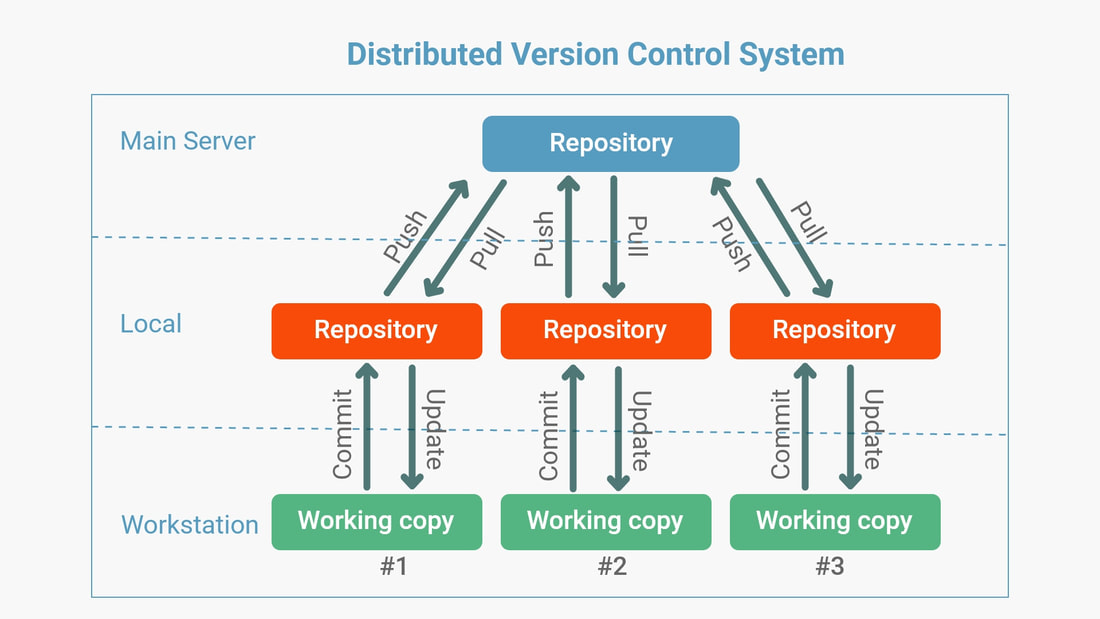
\includegraphics[width=0.85\textwidth]{distributed-vcs-structure}
    \caption{Distributed Version Control System (DVCS)}
    \label{fig:dvcs-structure}
\end{figure}

\subsubsection{Git}
\label{sec:git}
Git, created in 2005 by Linus Torvalds (also the creator of Linux), is primarily written in C with some shell scripts. Git was initially developed for the Linux codebase and has since become the most popular VCS in use today due to its features, flexibility, and speed. Torvalds explains that Git is a robust set of tools with many options, and its usage is often determined by what works best for collaboration rather than technical limitations.
% \smallskip

\begin{quote}
    "You can do a lot of things with Git, and many of the rules of what you should do are not so much technical limitations but are about what works well when working together with other people. So Git is a very powerful set of tools, and that can not only be overwhelming at first, it also means that you can often do the same (or similar) things different ways, and they all 'work.'" -- Linus Torvalds \cite{cloer_2019}
\end{quote}
% \smallskip

Git repositories are commonly hosted on local servers and cloud services, forming the backbone of a broad set of DevOps tools available from popular service providers, including GitHub, BitBucket, GitLab, and many others \cite{stopak_2019}.
\paragraph{Architecture}
\hfill\medskip\\
As a \nameref{sec:dvcs}, Git ensures that no repository copy needs to be designated as the centralised copy—instead, all copies are created equal. This contrasts with second-generation VCS, which relies on a centralised copy for users to check in and out.
\smallskip

This design allows developers and coding partners to share changes directly with each other before merging their changes into an official branch, fostering a flexible distributed workflow for team collaboration.
\smallskip

Moreover, developers can commit changes to their local copy of the repository without other repositories knowing about it. This enables commits without a network or internet connection, allowing developers to work offline until they are ready to push their changes to other repositories for review, testing, or deployment.
\smallskip

When a file is added for tracking with Git, it is compressed using the \lstinline{zlib} compression algorithm and hashed using a \lstinline{SHA-1} hash function \cite{stopak_2019}. This generates a unique hash value corresponding to the file content, which Git stores in an object database located in the hidden \lstinline{.git/objects} folder. These files, called \lstinline{Git blobs}, are created each time a new file (or a changed version of an existing file) is added to the repository.
\smallskip

Git uses a staging index that functions as a temporary space for changes being readied for a commit. When changes are set to be committed, their compressed data is referenced in a unique index file, appearing as a tree object. \lstinline{Trees} in Git link blob objects to actual file names, file permissions, and connections to other trees, signifying the status of a specific collection of files and directories. After all associated changes have been staged for commit, the index tree can be committed to the repository, generating a commit object within the Git object database \cite{stopak_2019}.
\smallskip

A commit denotes the primary tree for a specific revision, and the commit author, email address, date, and a descriptive commit message. Each commit also retains a reference to its preceding commit/commits, constructing a record of the project's evolution.
\smallskip

Git objects, including blobs, trees, and commits, are all compressed, hashed, and saved in the object database based on their respective hash values. These standalone objects avoid using diffs for space conservation, making Git highly efficient since the complete content of every file revision is readily available as an individual object.

% TODO: 2023-04-18
% \smallskip

% Nonetheless, particular operations, such as pushing commits to a remote repository, storing an excessive number of objects, or manually executing Git's garbage collection command, may prompt Git to reorganise objects into pack files. This packing procedure compresses inverse diffs to remove duplicate content and minimise size. This leads to the creation of \lstinline{.pack} files containing the object data, each paired with a corresponding \lstinline{.idx} (index) file that references the packed objects and their positions within the pack file. These pack files are transmitted across the network when branches are pushed to or fetched from remote repositories. When pulling or retrieving branches, the pack files are decompressed to generate loose objects in the object repository.

% ==============================================================================

% TODO: Consider adding command examples
% \paragraph{Basic Commands}

% \begin{itemize}
%     \item \lstinline{git init} - Initialize a Git repository in the current directory (creates the hidden \lstinline{.git} folder and its contents).
%     \item \lstinline{git clone <git-url>} - Download a copy of the Git repository at the specified URL.
%     \item \lstinline{git add <filename.ext>} - Add an untracked file or changed file to the staging area (creates corresponding entries in the object database).
%     \item \lstinline{git commit -m 'Commit message'} - Commit a set of changed files and folders along with a descriptive commit message.
%     \item \lstinline{git status} - Show information related to the state of the working directory, current branch, untracked files, modified files, etc.
%     \item \lstinline{git branch <new-branch>} - Create a new branch based on the current checked-out branch.
%     \item \lstinline{git checkout <branch>} - Checkout the specified branch into the working directory.
%     \item \lstinline{git merge <branch>} - Merge the specified branch into the current branch checked-out in the working directory.
%     \item \lstinline{git pull} - Update the working copy by merging in committed changes that exist in the remote repository but not the working copy.
%     \item \lstinline{git push} - Pack loose objects for local active branch commits into pack files and transfer to remote repository.
%     \item \lstinline{git log} - Show the commit history and associated descriptive messages for the active branch.
%     \item \lstinline{git stash} - Save all uncommitted changes in the working directory to a cache so that they can be retrieved later.
% \end{itemize}

% ==============================================================================
\subsubsection{Mercurial}
\label{sec:mercurial}
Mercurial, created in 2005 by Matt Mackall and written in \lstinline{Python}, initially aimed to host the codebase for Linux, but \nameref{sec:git} was chosen instead \cite{stopak_2019}. As the second most popular distributed VCS after Git, Mercurial is used far less frequently.
\paragraph{Architecture}
\hfill\medskip\\
Comparable to \nameref{sec:git}, Mercurial is a \nameref{sec:dvcs} that enables multiple developers to work on seperate copies of the same project. Although Mercurial utilises many similar technologies as \nameref{sec:git}, such as compression and \lstinline{SHA-1} hashing, it does so in distinct ways.
\smallskip

When a new file is tracked in Mercurial, a corresponding \lstinline{revlog} (revision log) file is generated for it in the hidden \lstinline{.hg/store/data/} directory. \lstinline{Revlog} files can be viewed as advanced versions of the history files employed by older \acrshortpl{vcs} such as \nameref{sec:cvs}, \nameref{sec:rcs}, and \nameref{sec:sccs}.
\smallskip

Unlike \nameref{sec:git}, which generates a new blob for each version of every staged file, Mercurial merely creates a new entry in the revlog for that file. To conserve space, each new entry contains only the delta (modifications) from the preceding version. Once a certain number of deltas is achieved, a complete snapshot of the file is stored again, minimising lookup time when applying numerous deltas to reconstruct a specific file revision.

% TODO: 2023-04-18
% \smallskip

% These file revlogs are named to correspond with the files they monitor but are postfixed with \lstinline{.i} and \lstinline{.d} extensions. The \lstinline{.d} files hold the compressed \lstinline{delta} content, while the \lstinline{.i} files function as \lstinline{indexes} to locate distinct revisions within the \lstinline{.d} files swiftly. For small files with few revisions, both the \lstinline{indexes} and \lstinline{content} are stored in \lstinline{.i} files. Revlog file entries are compressed for efficiency and hashed for identification, with the hash values referred to as \lstinline{nodeids}.
% \smallskip

% When a new commit is made, Mercurial tracks all file revisions in that commit using a manifest, which is also a revlog file. Rather than storing individual file content like the file revlogs, the manifest stores a list of filenames and \lstinline{nodeids} that specify which file revision entries exist in each project revision. These manifest entries are also compressed and hashed, with the hash values once more referred to as \lstinline{nodeids}.
% \smallskip

% Lastly, Mercurial employs one additional type of revlog called a \lstinline{changelog}. The \lstinline{changelog} contains a list of entries that associate each commit with the following details:
% \begin{itemize}
%     \item \lstinline{Manifest nodeid} - Identifies the complete set of file revisions that exist at a specific time.
%     \item \lstinline{Parent commit nodeid(s)} - Enables Mercurial to construct a timeline or branch of project history. One or two parent IDs are stored depending on the commit type (normal vs merge).
%     \item \lstinline{Commit author} - The name of the person who made the commit.
%     \item \lstinline{Commit date} - The date and time the commit was made.
% \end{itemize}


% ==============================================================================

% TODO: Consider adding command examples
% \paragraph{Basic Commands}
% \begin{itemize}
%     \item \lstinline{hg init} - Initialize the current directory as a Mercurial repository (creates the hidden \lstinline{.hg} folder and its contents).
%     \item \lstinline{hg clone <hg-url>} - Download a copy of the Mercurial repository at the specified URL.
%     \item \lstinline{hg add <filename.ext>} - Add a new file for revision tracking.
%     \item \lstinline{hg commit -m 'Commit message'} - Commit a set of changed files and folders along with a descriptive commit message.
%     \item \lstinline{hg status} - Show information related to the state of the working directory, untracked files, modified files, etc.
%     \item \lstinline{hg update <revision>} - Checkout the specified branch into the working directory.
%     \item \lstinline{hg merge <branch>} - Merge the specified branch into the current branch checked out in the working directory.
%     \item \lstinline{hg pull} - Download new revisions from remote repository but don't merge them into the working directory.
%     \item \lstinline{hg push} - Transfer new revisions to remote repository.
%     \item \lstinline{hg log} - Show the commit history and associated descriptive messages for the active branch.
% \end{itemize}

% ==============================================================================
% \subsubsection{BitKeeper}
% % TODO: Explain BitKeeper
% \newpage
% \newpage
% % \subsubsection{Darcs Advanced Revision Control System (Darcs)}
% % % TODO: Explain Darcs
% % \subsubsection{Monotone}
% % % TODO: Explain Monotone
% % \newpage
% % \newpage
% \subsubsection{Bazaar}
% \label{sec:bazaar}
% % TODO: Explain Bazaar
% \newpage
% \newpage
% \subsubsection{Fossil}
% % TODO: Explain Fossil
% \newpage
% \newpage
% ==============================================================================
% TODO: Discuss key features for a VCS
% \section{Summary of Key Features}
% \noindent
% \subsection{Repositories}
% % TODO: Explain repositories
% \subsection{Commits}
% \newpage
% % TODO: Explain commits
% \subsection{Branching and Merging}
% % TODO: Explain branching and merging
% \newpage
% \subsection{Pulling and Pushing}
% % TODO: Explain pulling and pushing
% \newpage
